\chapter{Analyzing CxAnalytix Data}

CxAnalytix outputs data related to vulnerabilities as they are detected and remediated over time.  This means the data collected can be classified as 
\href{https://en.wikipedia.org/wiki/Time_series}{time-series data}.  Time series data, as a basic definition, is periodically recording values that change over time.  
Each recorded value can be referred to as a "sample".

\noindent\\This generally causes some confusion as most people are accustomed to analyzing business data that essentially only records the current state of 
the business (e.g. "Give me a A/R report showing me a list of customers that have outstanding balances, grouping the past-due amounts in 30/60/90 day buckets.")  
Most of this data is organized in a relational form that is selected by understanding the relational linkage between multiple entities.  The pre-requisite for
extracting meaning from data organized relationally would be to understand which entities are related.

\noindent\\The CxAnalytix data is generally "flat" output (with a few exceptions); this means there is no knowledge required to understand the relationship between entities.
Each record (or "sample") has all values required for the context of the record without needing to understand any relationships between entities.  The technique for
deriving meaning from the data is to understand the filtering criteria needed to reduce the data set to show only the data needed for analysis.  Often this filtering is
performed as a pipeline starting with the widest filtering criteria sending data through progressively narrower filtering criteria.

\subsection{Understanding Sampling Behavior}

Performing analysis on vulnerability data requires a bit of knowledge about the circumstances by which data arrives.  Most time series data is collected from 
sensors that are emitting samples on a somewhat predictable periodic basis; vulnerability data is not collected in the same manner. Vulnerability scans are not 
necessarily performed with a predictable cadence.  There are some reasons for this:


\begin{itemize}
    \item Scanning code on commit to a repository would require commits to a repository; developers don't always work on code in a particular repository, 
    and they certainly do not have a regular pattern for committing code.
    \item Scheduled scans may fail or be delayed by lack of scanning resources.
    \item Ad-hoc scans may be interleaved between scans scheduled on a regular cadence.
    \item Code that is not under active development may not get scanned regularly.
\end{itemize}


\subsection{Factors Influencing Result Changes}

There are several variables that affect how vulnerabilities can change over time.  The most obvious one is that vulnerabilities appear and disappear based on code
changes as development is performed over time.  If this were the only factor that caused changes in detected vulnerabilities, analysis would be easy. Consider:

\begin{itemize}
    \item Upgrades to the SAST software can increase the coverage of languages, frameworks, APIs, and even coding techniques.  Vulnerability count trends may
    reflect the level of scan accuracy that product changes introduce in the upgrade.
    \item Tuning of the Preset, Exclusions, and/or CxQL query can change what is detected in a scan.
    \item The submitted code can be changed to affect the scan results.
    \item In some integration scenarios, it is possible for developers to submit code to exclude files containing vulnerable code. The issue will appear
    to have been remediated due to a change in the build process that can not be observed by static code analysis.
    \item Similarly, it is possible to inadvertently submit code that should not be scanned thus increasing the number of results.
    \item Errors in the management of the code may cause vulnerabilities that were previously fixed to reappear.
    \item Incremental scan results will likely differ significantly from full scan results.
\end{itemize}


\subsection{Identifying SAST vulnerabilities over Multiple Scans}

The SAST Vulnerability Detail records have every node for every path in the reported vulnerabilities.  Often filtering the data where \texttt{NodeId == 1}
is sufficient to reduce the amount of data that needs to be considered.  Uniquely identifying a vulnerability can be done by calculating a
"fingerprint" for the vulnerability.

\noindent\\Most approaches make the wrong assumption that \texttt{SimilarityId} can be used to identify each vulnerability across scans.  This does not work due to:

\begin{itemize}
    \item Vulnerability paths for files that are copied to different paths will have the same \texttt{SimilarityId}.
    \item Vulnerability paths for files that are scanned in multiple projects will have the same \texttt{SimilarityId}.
    \item Code that is copy/pasted multiple times in the same file may have the same \texttt{SimilarityId}.
    \item Different vulnerabilities with the same start and end node in the data flow path will have the same \texttt{SimilarityId}.
\end{itemize}


\noindent\\Identifying a specific vulnerability across scans can be done by hashing a compound identifier generated from fields in the data record. To understand 
which components to select for the compound identifier, some explanation of how record data elements can be used to derive a fingerprint is required.

\subsubsection{Project Identification}

Scans are executed under the context of a SAST project; in most cases, this SAST project represents a collection of scans over the lifetime of code evolution
for code in a single repository. \texttt{ProjectId} would therefore be a unique, non-changing value suitable for establishing a logical collection
of related scan data.

\noindent\\Another option for identifying a logical collection of related scan data would be to concetenate \texttt{TeamName} and \texttt{ProjectName} as a path.  
For example, "/CxServer/US/FinancialServices/ShoppingCart\_master" has a team name of "/CxServer/US/FinancialServices" and a project name of "ShoppingCart\_master".
This is roughly equivalent to the uniqueness of \texttt{ProjectId}, with the caveat that projects can be re-assigned to a different team.  If a project is assigned
to a different team, it is logically no longer the same project for the purposes of tracking scans over the lifetime of code scanned in the SAST project.  If your
analysis needs are to track vulnerabilities on a team level, using \texttt{TeamName} and \texttt{ProjectName} for a unique identifier may be better suited as
a way to identify a logical grouping of scans.

\noindent\\It is important to note that SAST treats vulnerabilities with the same \texttt{SimilarityId} as a single vulnerability across all projects in the same team.  
Setting a vulnerability with the status of \textbf{Not Exploitable} in one project, for example, would result in the vulnerability being marked 
as \textbf{Not Exploitable} if the same file (or a copy of it) were scanned in another project on the same team.


\subsubsection{Vulnerability Classification}

Since vulnerabilities may have the same start and end node, the \texttt{SimilarityId} value may appear under multiple vulnerability categories 
(or even multiple times per category).  The category roughly corresponds to the \texttt{QueryName}.  Often, the use of \texttt{QueryName} as a component in a 
compound identifier would be sufficient for classification since most queries won't report results for the same \texttt{QueryName} that appear in a 
different \texttt{QueryGroup} with the same \texttt{SimilarityId}.  This is usually the case given the result path is limited to a single language in all nodes of the
data flow path.

\noindent\\It is possible, however, to have language agnostic results (such as those generated by TruffleHog) that give the same result for the same 
\texttt{QueryName} under each \texttt{QueryGroup}.  Using both the \texttt{QueryGroup} and \texttt{QueryName} as part of the compound identifier would increase the 
uniqueness accuracy.

\subsubsection{Aggregation of Data from Multiple SAST Instances}

If you have multiple SAST instances and are aggregating the data into a single store, consider using \texttt{InstanceId} to compose the vulnerability fingerprint.  Data
from multiple SAST instances implies that \texttt{ProjectId} is no longer unique.

\subsubsection{Examples of Vulnerability Fingerprints}\label{sec:fingerprint}
It is important to note that code changes over time but may remain vulnerable to the same detected vulnerability.  Code format and composition affect
the ability to uniquely identify a vulnerability algorithmically.  A human may look at code changes and understand that it is the same code, but identifying
it is the same code algorithmically is significantly more complicated.  Identifying exact uniqueness of a particular vulnerability requires virtually no code changes
over time; this is not a realistic expectation for code under active development.  Code that is actively developed, however, is generally changed in small 
increments between scans.  The fingerprinting methods described here are intended to generate a unique identifier that is sufficiently unique for the purpose of 
tracing the lifecycle of a specific vulnerability.

\noindent\\It is important to note that using the fingerprint as a method for counting the number of vulnerabilities may result in differences between
the number of reported vulnerabilities in SAST scan summary views and project dashboards.  This is due to the occasional coalescing of duplicate vulnerabilities
into a single fingerprinted vulnerability.  This is generally seen when multiple vulnerabilities are reported for code that has been duplicated in multiple
locations in the scanned code.


\textbf{\noindent\\\\Fingerprint Composition: \texttt{ProjectId} + \texttt{QueryName} + \texttt{SinkFileName} + \texttt{SinkLine} + \texttt{SimilarityId}}

\noindent\\This fingerprint is generally suitable for tracking a vulnerability across multiple scans in a SAST project.    

\noindent\\For greater accuracy in tracking, consider adding the following fields:

\begin{itemize}
    \item \texttt{QueryGroup}
    \item \texttt{QueryLanguage} + \texttt{QuerySeverity}
    \item \texttt{QueryLanguage} + \texttt{ResultSeverity}
\end{itemize}

\textbf{\noindent\\\\Fingerprint Composition: \texttt{TeamName} + \texttt{QueryName} + \texttt{SinkFileName} + \texttt{SinkLine} + \texttt{SimilarityId}}

\noindent\\Using \texttt{TeamName} in place of \texttt{ProjectId} will effectively allow vulnerabilities to be assessed once for all projects assigned to a team.  There 
are some potential drawbacks to this approach:

\begin{itemize}
    \item The same code in unrelated projects may be counted as one vulnerability for all projects in the team.
    \item Projects can be moved to different teams.  Moving a project to a new team will change the timeline for the vulnerability given
    historical samples will reflect the team name at the time the sample was recorded.
    \item It may not be possible to determine when a vulnerability was resolved since it will require all projects in the team that report the
    vulnerability to perform a scan that no longer contains the vulnerability.  
\end{itemize}




\subsection{Counting Vulnerabilities}\label{sec:counting}

\subsubsection{SAST Reported Counts}

The vulnerability counts that can be obtained via the SAST UI show counts of High, Medium, Low, and Informational vulnerabilities that have any state other
than \textbf{Not Exploitable}.  

\noindent\\As scan results are triaged, any vulnerabilities marked as \textbf{Not Exploitable} will cause the count to be recalculated
to subtract the vulnerabilities with the changed state.  This will also apply to all historical scans; viewing the summary of a historical scan
will show a count that reflects changes made to vulnerabilities that have been reported in multiple scans.  The recalculation also affects the risk score of
historical scans that is displayed in the list of scans for the project.  The recalculation is generally performed within a few minutes of the result state being recalculated.

\noindent\\The CxAnalytix Scan Summary Record currently reports a total of all vulnerabilities, regardless of the state of the vulnerability.  As of the writing of this manual,
this is considered a defect.  Future versions of CxAnalytix will calculate vulnerability counts by not considering vulnerabilities marked as \textbf{Not Exploitable}.


\subsubsection{Counting with Scan Detail Record}

It is possible to recreate the same counting logic as SAST by filtering the detail records where \texttt{NodeId == 1} and \texttt{State != 1}.  The \texttt{State}
numeric values correspond to the following result states:


\begin{itemize}
    \item 0 = To Verify
    \item 1 = Not Exploitable
    \item 2 = Confirmed
    \item 3 = Urgent
    \item 4 = Proposed Not Exploitable
\end{itemize}

\noindent\\It is often the case that there is a need to calculate triaged vs. untriaged vulnerability counts.  The triage state \texttt{To Verify} is the
initial state for all vulnerabilities upon detection.  The state value of each vulnerability can be used as filtering or grouping options to derive appropriate counts.


\subsubsection{Counting by Fingerprint}

As noted in Section \ref{sec:fingerprint}, the fingerprint can coalesce similar vulnerabilities into a single fingerprint.  Some opinions may considered this problematic for
counting purposes. 

\noindent\\The reason for coalescing is usually due to a duplicate \texttt{SimilarityId} for multiple reported data flow paths. Fingerprinted vulnerabilities coalesce into a 
single vulnerability when duplicate \texttt{SimilarityId} values cause the fingerprint calculation to yield the same fingerprint.  Vulnerabilities with the same 
\texttt{SimilarityId} are treated as the same vulnerability in SAST, even if each reported vulnerability flows through different code or exists in different files.  
This is mostly observed when triage changes for a vulnerability propagate across all projects on a team.

\noindent\\There are many reasons why duplicate \texttt{SimilairtyId} values will be generated. Copy/paste code, while not common in most code, can generate duplicate 
\texttt{SimilarityId} data flows.  The duplicate data flows often occur when:

\begin{itemize}
    \item The source and sink nodes for multiple distinct paths are the same.
    \item The source and sink nodes contain code that is the same.
\end{itemize}

\noindent\\As an example, consider this code sample that produces 3 SQL Injection vulnerabilties:

\begin{code}{}{}{}
using System;
using System.Collections.Generic;
using System.Linq;
using System.Threading.Tasks;
using Microsoft.AspNetCore.Mvc;
using Microsoft.AspNetCore.Mvc.RazorPages;
using System.Data.SqlClient;
using System.IO;
using System.Text;

namespace webapp.Pages
{
    public class IndexModel : PageModel
    {

        private String getField(String[] fields, int index)
        {
            return Request.Form[fields[index]];
        }


        public void OnPost()
        {

            String[] fieldNames = {"A", "B", "C"};
            int curField = 0;
                        
            SqlConnection con = new SqlConnection();

            String response = String.Empty;
            String dbData = null;
            
            dbData = new SQLCommand($"SELECT * FROM SomeTable WHERE SomeColumn = '{getField(fieldNames, curField)}'", con).ExecuteScalar();
            if (dbData != null)
              response += $"Field A: {dbData}<P>";
            
            curField++;

            dbData = new SQLCommand($"SELECT * FROM SomeTable WHERE SomeColumn = '{getField(fieldNames, curField)}'", con).ExecuteScalar();
            if (dbData != null)
              response += $"Field B: {dbData}<P>";

            curField++;

            dbData = new SQLCommand($"SELECT * FROM SomeTable WHERE SomeColumn = '{getField(fieldNames, curField)}'", con).ExecuteScalar();
            if (dbData != null)
              response += $"Field C: {dbData}<P>";
            
            Response.Body.Write(new ReadOnlySpan<byte>(Encoding.UTF8.GetBytes (response.ToArray ()) ) );
        }
    }
}

\end{code}

\noindent\\The SQL Injection vulnerabilties have the same source line and a unique sink line, but the \texttt{SimilarityId} is the same for all vulnerabilities.  
This means that a triage change for only one vulnerabilitiy will apply it to all vulnerabilities with the same \texttt{SimilarityId}.  Reviewing the XML report of the 
code example confirms the \texttt{SimilarityId} is the same for all SQL Injection data flow paths:

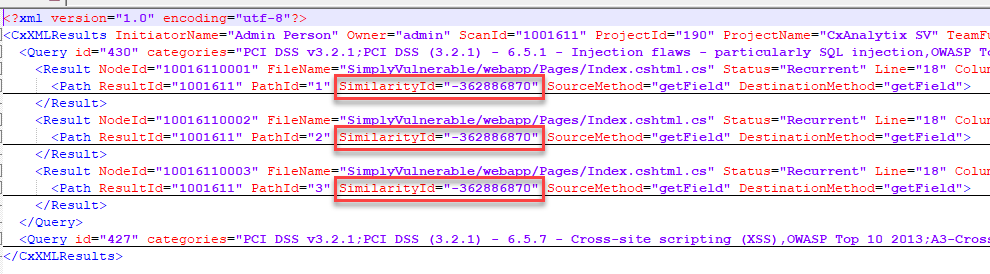
\includegraphics[scale=.6]{graphics/Data-Analysis-FAQ-SimId-XML.png}

\subsection{Counting New/Resolved/Recurrent Vulnerabilities}

To obtain only deltas of vulnerability counts between scans to track changes, uniquely identifying vulnerabilities is likely not required.  Section \ref{sec:counting}
details various methods of counting vulnerabilities.  Applying the counting logic to the latest scan and the previous scan is one method of yielding data needed to
calculate the change delta between scans.


\subsubsection{Calculating New Vulnerability Counts}

The \texttt{Status} field in the SAST Vulnerability Details record will have the value \textbf{New} to indicate the vulnerability has been detected for the first time in 
a scan for the project.

\noindent\\\texttt{Status} with the value of \textbf{Recurrent} means that this vulnerability has been reported previously for one or more scans in the same project.  
The vulnerability could be added to the most recent scan but still have the \textbf{Recurrent} status under some conditions:

\begin{itemize}
    \item The vulnerability was previously remediated and then re-introduced into the code.
    \item Preset changes removed a query from previous scans before being changed again to add the query back into the latest scans.
    \item Exclusion adjustments change the scope of scanned code and removed the vulnerable code from a prior scan before being adjusted again to add the code back
    into recent scans.
\end{itemize}


\subsection{Determining when a Vulnerability was First Detected}

The easiest method is to find the vulnerability where the \texttt{Status} field is \textbf{New}.  This works if and 
only if a sample was recorded the first time the vulnerability was detected.  There are various scenarios where this may not happen:

\begin{itemize}
    \item The report for the scan could not be retrieved at the time CxAnalytix performed the crawl for scans.
    \item Data retention has been run and the first scan was purged prior to CxAnalytix crawling the scans.
\end{itemize}

A more general method may be to use the compound identifier for tracking vulnerabilities across scans and determine which scan is associated with the 
sample containing the earliest value in the \texttt{ScanFinished} field.

\subsubsection{FirstDetectionDate}

As of SAST 9.3 and CxAnalytix 1.3.1, the field \texttt{FirstDetectionDate} is part of the data output specification.  Scans executed prior to 9.3 will not have a true
value for \texttt{FirstDetectionDate}.  


\subsection{Detecting when a Vulnerability has been Resolved}

This depends on how your organization defines the criteria for a "resolved vulnerability".  There will be two methods of determining how to find the date
for vulnerability resolution that should fit for most definitions of a "resolved vulnerability".


\noindent\\To explain, some variable definitions are required:\\
\begin{itemize}
    \item Let $V_T$ be the vulnerability that is tracked across multiple scans using the chosen composite identifier.
    \item Let $\mathbb{S}$ be the set of scans having the same \texttt{ProjectId} field value where at least one scan reports $V_T$.
    \item Let the subset $\mathbb{S}_{found}$ be the subset of scans where $V_T$ is reported
    such that $\mathbb{S}_{found} = \{\mathbb{S} | V_T \text{ is reported}\}$ and $\mathbb{S}_{found}\subseteq\mathbb{S}$
\end{itemize}

\noindent\\Finding the date $V_T$ first appeared means finding scan
$S_{found}\in\mathbb{S}_{found}$
with the earliest value for \texttt{ScanFinished}.

\subsubsection{The Easy Method}

Given the subset of scans where $V_T$ is not reported 
$\mathbb{S}_{fixed}= \{\mathbb{S} | \text{not reporting }V_T\}$ 
we know that if $\mathbb{S}_{fixed} == \varnothing$ (empty set) that the vulnerability is still outstanding.  

\noindent\\If the most recent scan $\text{S}_{latest}\in\mathbb{S}$ is also in $\mathbb{S}_{fixed}$ ($\text{S}_{latest}\in\mathbb{S}_{fixed}$), then we can find the scan
$\text{S}_{fixed}\in\mathbb{S}_{fixed}$ with the earliest \texttt{ScanFinished} date to find the date
the vulnerability was remediated.

\subsubsection{The Hard Method}

Note that it is possible for $V_T$ to be re-introduced to the code; while it may be rare, the result is that there are potentially multiple 
resolution dates. If $\text{S}_{fixed}\notin\mathbb{S}_{fixed}$, it can be assumed that the vulnerability was re-introduced and is still outstanding. 

\noindent\\The detection method presented above will technically work for all cases at the expense of the accuracy of dates related to appearance and resolution.  Your organization
can decide how they would like to approach analysis for this case.  If there is a need to find a more exact date of resolution, more advanced logic is needed.

\noindent\\For a basic method of dealing with vulnerability reappearance, the \texttt{ScanFinished} date for 
$\text{S}_{found}$ may still be considered the date $V_T$ first appeared for most tracking purposes. It must still hold 
that $\text{S}_{latest}\in\mathbb{S}_{fixed}$ to indicate the vulnerability has been resolved.

\noindent\\Using the scan $\text{S}_{most-recent-found}\in\mathbb{S}_{found}$ where the \texttt{ScanFinished} value is the most recent is the date where the search for
the latest fix date can begin.

\noindent\\Find the scan where $V_T$ was most recently fixed $\text{S}_{most-recent-fixed}\in\mathbb{S}_{fixed}$
by selecting 
$\text{S}_{most-recent-fixed}$ with a \texttt{ScanFinished} value greater than that of 
the \texttt{ScanFinished} value of $\text{S}_{most-recent-found}$
\textbf{and} the earliest value for all scans
$\text{S}\in\mathbb{S}_{fixed}$.
The \texttt{ScanFinished} value for $\text{S}_{most-recent-fixed}$ is the latest date on which
$V_T$ was resolved.

\subsubsection{Additional Considerations}

As the code changes from scan to scan, it is possible the fields used in creating a fingerprint for the vulnerability may also change.  Changes in the fingerprint may 
lead to the assumption that the vulnerability is "closed" since the vulnerability no longer appears in the scan.  A new vulnerability will then appear as "open" given 
the new fingerprint has appeared.

\noindent\\SAST assigns the \texttt{FirstDetectionDate} the \texttt{SimilarityId} of the result.  A scan may have multiple vulnerabilities reported having the 
same \texttt{SimilarityId}, therefore these results have the same \texttt{FirstDetectionDate}.  

\noindent\\Methods for tracking the lifecycle of the vulnerability for the purpose of setting a resolution SLA may need to consider this information to understand
if SLA aging resets as code changes.  In many cases, the use of the fingerprint is sufficient given that code may not change often enough to perpetually reset SLAs.


\subsection{Project Information Records}

The Project Information record is a sample of the current state of a project.  The fields indicate the state of the project at the time CxAnalytix performed the 
crawl each project.  Often the project information does not change between scans, therefore it will appear as if the project information is duplicated.

\noindent\\If a project has had no scans executed since the previous crawl, there is effectively no change that has been imposed on the project.  If there are
no changes for the project, there is no project information recorded.  If one or more
scans are executed since the previous crawl, the a Project Information sample will be recorded for the crawl.

